% questions.tex —— 1982 年·全国卷（理科） · 题目内容片段（无答案）
% 由 tools/generate_projects.py 依来源总账自 1982/1982_数学真题_理_试题.md 生成，勿手改（改源 MD 后重跑）


\begin{gktip}
\textbf{来源说明}：本卷为固定原卷《1982理.pdf》单页（原卷页码第 19 页），系 1982 年全国统一招生考试理科卷；同年另有文科卷，二者题目不同。全卷共 8 题，卷末另有「附加题」栏一题，原卷沿用大题号印作「9．」，本库作为附加题 9 保留在第 8 题之后，不计入正式题量。原卷未标注分值，题面亦不含答案（答案由本库独立推导）。

\textbf{转录说明}：本代 PDF 的文本层会丢根号与分数线，本文一律按 PDF 页面图像转录；第 1 题为表格题，原表第三列供填答，此处照录为空白；第 4、6、7 题依原卷配图重绘为 TikZ 矢量图。
\end{gktip}

\begin{question}
\gkti{1}填表：

\begin{center}
\begin{tabular}{lll}
\toprule
 & 函数 & 使函数有意义的 $x$ 的实数范围 \\
\midrule
1 & $y=\sqrt{-x^2}$ &  \\
2 & $y=\sqrt{(-x)^2}$ &  \\
3 & $y=\arcsin(\sin x)$ &  \\
4 & $y=\sin(\arcsin x)$ &  \\
5 & $y=10^{\lg x}$ &  \\
6 & $y=\lg 10^x$ &  \\
\bottomrule
\end{tabular}
\end{center}

\end{question}
\begin{question}
\gkti{2}

（1） 求 $(-1+\mathrm i)^{20}$ 展开式中第 15 项的数值；

（2） 求 $y=\cos^2\dfrac{x}{3}$ 的导数。

\end{question}
\begin{question}
\gkti{3}在平面直角坐标系内，下列方程表示什么曲线？画出它们的图形。

\Needspace{5\baselineskip}
（1） 
\nopagebreak[4]
\[
\begin{vmatrix}
2x & 1 & 1\\
-3y & 2 & 3\\
6 & 3 & 4
\end{vmatrix}=0;
\]

\Needspace{5\baselineskip}
（2） 
\nopagebreak[4]
\[
\begin{cases}
x=1+\cos\varphi\\
y=2\sin\varphi
\end{cases}
\]

\Needspace{0.4\textheight}
\end{question}
\begin{question}
\gkti{4}已知圆锥体的底面半径为 $R$，高为 $H$，求内接于这个圆锥体并且体积最大的圆柱体的高 $h$（如图）。
\nopagebreak[4]
\begin{center}% 1982 年全国卷（理科）第 4 题：圆锥及其内接体积最大的圆柱（按源卷布局）。
% 底面半径 R=2.0、高 H=3.4；圆柱底半径 r=0.6、高 h=2.38（源卷约取全高的 0.7）。
% 右侧为 H、h 的尺寸线（均自锥底量起），下方为 2R 的尺寸线。
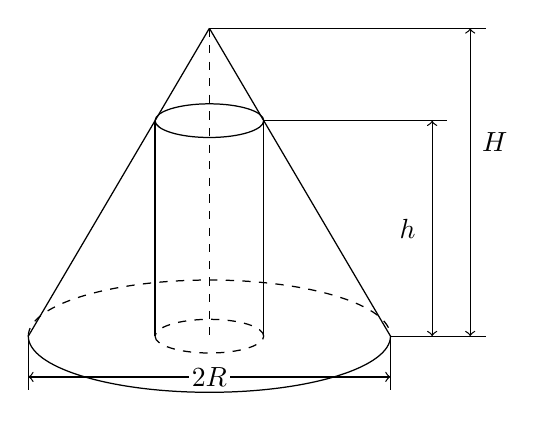
\begin{tikzpicture}[scale=1.15, line width=0.45pt,
  every node/.style={inner sep=1.5pt}]
  % 圆锥底面椭圆（半轴 2.0 与 0.62）：前半（近观者）实线，后半虚线
  \draw (-2.0,0) arc (180:360:2.0 and 0.62);
  \draw[dashed] (-2.0,0) arc (180:0:2.0 and 0.62);
  % 圆锥母线
  \draw (0,3.4) -- (-2.0,0);
  \draw (0,3.4) -- (2.0,0);
  % 圆锥轴（虚线）
  \draw[dashed] (0,3.4) -- (0,0);
  % 圆柱侧面轮廓母线
  \draw (-0.6,0) -- (-0.6,2.38);
  \draw (0.6,0) -- (0.6,2.38);
  % 圆柱上底面（可见，实线椭圆，半轴 0.6 与 0.186）
  \draw (-0.6,2.38) arc (180:360:0.6 and 0.186);
  \draw (0.6,2.38) arc (0:180:0.6 and 0.186);
  % 圆柱下底面（被遮，虚线椭圆）
  \draw[dashed] (-0.6,0) arc (180:360:0.6 and 0.186);
  \draw[dashed] (0.6,0) arc (0:180:0.6 and 0.186);
  % 右侧尺寸线：H 为锥高、h 为圆柱高，均自锥底量起
  \draw (0,3.4) -- (3.05,3.4);
  \draw (2.0,0) -- (3.05,0);
  \draw (0.6,2.38) -- (2.62,2.38);
  \draw[<->] (2.88,0) -- (2.88,3.4);
  \node[right] at (2.96,2.14) {$H$};
  \draw[<->] (2.46,0) -- (2.46,2.38);
  \node[left] at (2.33,1.19) {$h$};
  % 下方尺寸线 2R
  \draw (-2.0,0) -- (-2.0,-0.6);
  \draw (2.0,0) -- (2.0,-0.6);
  \draw[<->] (-2.0,-0.45) -- (2.0,-0.45);
  \node[fill=white, inner sep=1pt] at (0,-0.45) {$2R$};
\end{tikzpicture}
\end{center}
\nopagebreak[4]
\end{question}
\begin{question}
\gkti{5}设 $0<x<1$，$a>0$，$a\ne1$，比较 $\lvert\log_a(1-x)\rvert$ 与 $\lvert\log_a(1+x)\rvert$ 的大小。（要写出比较过程）

\Needspace{0.4\textheight}
\end{question}
\begin{question}
\gkti{6}如图：已知锐角 $\angle AOB=2\alpha$ 内有动点 $P$，$PM\perp OA$，$PN\perp OB$，且四边形 $PMON$ 的面积等于常数 $c^2$。今以 $O$ 为极点，$\angle AOB$ 的角平分线 $OX$ 为极轴，求动点 $P$ 的轨迹的极坐标方程，并说明它表示什么曲线。
\nopagebreak[4]
\begin{center}% 1982 年全国卷（理科）第 6 题：∠AOB 内动点 P 到两边作垂足 M、N（按源卷布局）。
% O 为极点、OX 为角平分线（极轴）；M—P—N 为 P 到两边的垂线段，图中不连 M—N。
\begin{tikzpicture}[scale=1.5, line width=0.45pt,
  every node/.style={inner sep=1.5pt}]
  \coordinate (O) at (0,0);
  \coordinate (A) at (3.77,2.45);     % OA，与 OX 约成 33°
  \coordinate (B) at (3.77,-2.45);    % OB，与 OX 约成 -33°
  \coordinate (X) at (3.90,0);        % 角平分线 OX
  \coordinate (P) at (2.83,0.65);     % 动点 P
  \coordinate (M) at (2.285,1.484);   % P 在 OA 上的垂足
  \coordinate (N) at (1.690,-1.097);  % P 在 OB 上的垂足
  \draw (O) -- (A);
  \draw (O) -- (B);
  \draw (O) -- (X);
  \draw (M) -- (P);
  \draw (P) -- (N);
  \node[left] at (O) {$O$};
  \node[right] at (A) {$A$};
  \node[right] at (B) {$B$};
  \node[right] at (X) {$X$};
  \node[above left] at (M) {$M$};
  \node[right] at (P) {$P$};
  \node[below left] at (N) {$N$};
\end{tikzpicture}
\end{center}
\nopagebreak[4]
\Needspace{0.4\textheight}
\end{question}
\begin{question}
\gkti{7}已知空间四边形 $ABCD$ 中 $AB=BC$，$CD=DA$，$M$、$N$、$P$、$Q$ 分别是边 $AB$、$BC$、$CD$、$DA$ 的中点（如图）。求证：$MNPQ$ 是一个矩形。
\nopagebreak[4]
\begin{center}% 1982 年全国卷（理科）第 7 题：空间四边形 ABCD 及各边中点 M、N、P、Q（按源卷布局）。
% A 在左、B 在上、C 在下、D 在右；M(AB)、N(BC)、P(CD)、Q(DA) 依次连成四边形 MNPQ。
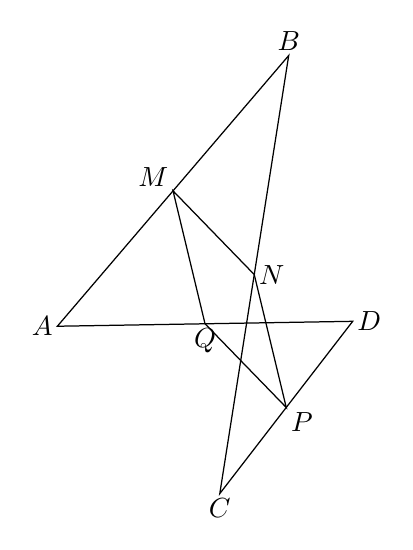
\begin{tikzpicture}[scale=1.25, line width=0.45pt,
  every node/.style={inner sep=1.5pt}]
  \coordinate (A) at (0,0);
  \coordinate (B) at (2.35,2.75);
  \coordinate (C) at (1.65,-1.70);
  \coordinate (D) at (3.00,0.05);
  \coordinate (M) at (1.175,1.375);   % AB 中点
  \coordinate (N) at (2.000,0.525);   % BC 中点
  \coordinate (P) at (2.325,-0.825);  % CD 中点
  \coordinate (Q) at (1.500,0.025);   % DA 中点
  % 空间四边形 ABCD
  \draw (A) -- (B) -- (C) -- (D) -- cycle;
  % 中点四边形 MNPQ
  \draw (M) -- (N) -- (P) -- (Q) -- cycle;
  \node[left] at (A) {$A$};
  \node[above] at (B) {$B$};
  \node[below] at (C) {$C$};
  \node[right] at (D) {$D$};
  \node[above left] at (M) {$M$};
  \node[right] at (N) {$N$};
  \node[below right] at (P) {$P$};
  \node[below] at (Q) {$Q$};
\end{tikzpicture}
\end{center}
\nopagebreak[4]
\end{question}
\begin{question}
\gkti{8}抛物线 $y^2=2px$ 的内接三角形有两边与抛物线 $x^2=2qy$ 相切，证明这个三角形的第三边也与 $x^2=2qy$ 相切。

\textbf{附加题 9．} 已知数列 $a_1$，$a_2$，$\cdots$，$a_n$，$\cdots$ 和数列 $b_1$，$b_2$，$\cdots$，$b_n$，$\cdots$，其中 $a_1=p$，$b_1=q$，$a_n=pa_{n-1}$，$b_n=qa_{n-1}+rb_{n-1}$（$n\geqslant2$），（$p$，$q$，$r$ 是已知常数，且 $q\ne0$，$p>r>0$）。

（1）用 $p$，$q$，$r$，$n$ 表示 $b_n$，并用数学归纳法加以证明；

（2）求 $\lim\limits_{n\to\infty}\dfrac{b_n}{\sqrt{a_n{}^2+b_n{}^2}}$。

\end{question}